\section{Theoretische Grundlagen}
Der Lock-In-Verstärker ist ein Gerät, das ein Periodisches Signal von einer bestimmten Frequenz empfangen und erkennen kann.
Dabei haben Störsignale, einen nur geringen Einfluss auf die Messung des Signals.
% Vermutlich keine Subsection
%Aufbau
Der Lock-In-Verstärker filtert das von außen kommende Signal $U_\text{sig}$ in zwei Schritten.
Der erste Schritt ist ein Bandpassfilter.
Dieser filtert alle Frequenzen heraus, die sehr weit von der Signalfrequenz $\omega$ entfernt sind.
Dazu muss der Bandpassfilter auf die Signalfrequenz eingestellt sein, damit er die richtigen Frequenzen filtern kann.
Im zweiten Schritt wird die Signalspannung $U_\text{sig}$ mit einer Referenzspannung $U_\text{ref}$ vermischt.
$U_\text{ref}$ ist eine Rechteckschwingung, die die gleiche Frequenz hat wie das ursprüngliche Signal in $U_\text{sig}$.

\begin{figure}
    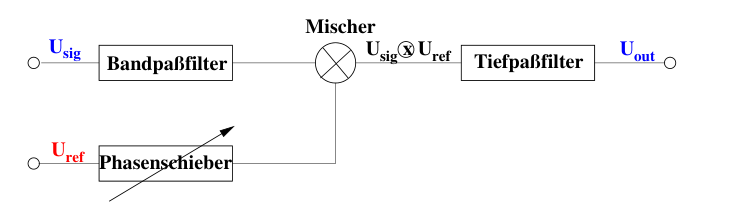
\includegraphics[width=\textwidth]{Abbildungen/Grundlegende_idee.png}
    \caption{Schematischer Aufbau des Lock-In-Verstärkers \cite[][]{man:v303}}
    \label{fig:grundlegende_Idee}
\end{figure}

